\documentclass[ordinary]{BMSTU-IU8}

\student{Н.В. Железцов}
\group{ИУ8-104}
\theme{
    Реферат на тему \\
    "Шифрование пользовательских данных Android устройства"
}

\discipline{Управление программными продуктами}
\supervisor{А.М. Карондеев}

\begin{document}
    \maketitle

    \tableofcontents
    \structure{ВВЕДЕНИЕ}

Целью практических занятий является изучение и освоение основных процедур
записи, обработки, измерения параметров и анализа характеристик речевого
сигнала с использованием современных программных средств.

Запись фонограммы выполнена с помощью программы Praat. Параметры записи:
частота дискретизации 11,025 кГц, разрядность 16 бит, режим «моно», формат wav.
Произносилась фраза: «Железцов Никита Владимирович, двадцать шестое марта две
тысячи двадцать пятого года. А, Э, И, О, У, Ы».

При анализе речевого сигнала и построении сонограмм использовались
программы Praat, Sound Edit, WaveView.


    \structure{ОСНОВНАЯ ЧАСТЬ}

\section*{Основы шифрования}

Конфиденциальность информации достигается за счет её шифрования. Шифрование
-- это преобразование информации с помощью криптографических алгоритмов.
Исходная информация -- это открытый, доступный для прочтения текст (открытый
текст, plaintext). После операции шифрования он превращается в зашифрованную
информацию -- т.е. бессмысленный набор символов (шифротекст, ciphertext). Для
его прочтения нужно провести операцию расшифрования -- т.е. восстановления
первоначального текста с использованием известного пользователю ключа
шифрования. Если ключ шифрования пользователю (атакующему) неизвестен, то
операция восстановления первоначального текста называется дешифрованием, и она
достигается за счет взлома шифра с использованием методов криптоанализа.

Криптографические алгоритмы шифрования делятся на две больших группы: алгоритмы
симметричного шифрования (криптосистемы с секретным ключом) и алгоритмы
асимметричного шифрования (криптосистемы с открытым и закрытым ключом).
Ключевая информация — это секретные ключи или пары открытых и закрытых ключей
(т.е. то, что может позволит зашифровать и расшифровать информацию). Важнейшей
характеристикой ключа шифрования является его длина, которая измеряется в
битах.

\begin{enumerate}
    \item Симметричное шифрование подразумевает использование одного и того же
        ключа и для шифрования, и для расшифрования. Такой ключ называется
        секретным ключом. Преимуществами симметричного шифрования являются
        скорость работы и меньшая длина ключа шифрования (по сравнению с
        алгоритмами асимметричного шифрования), а недостатки — это сложность
        безопасной передачи ключей в недоверенной среде (злоумышленник,
        перехвативший секретный ключ, сможет прочитать все сообщения,
        зашифрованные им) и сложность управления ключами (каждый секретный ключ
        приходится безопасно доставлять каждому отправителю и получателю и
        хранить у них). Алгоритмы симметричного шифрования делятся на потоковые
        (stream cipher) и блочные (block cipher):

    \begin{enumerate}
        \item Алгоритм симметричного потокового шифрования производит
            шифрование каждого символа (бита/байта) сообщения отдельно,
            выполняя математическую операцию XOR («исключающее ИЛИ») с ключом
            (ключевым потоком, гаммой). Преимуществами потокового шифрования
            являются его простота (что позволяет выполнять шифрование на
            оборудовании с невысокой вычислительной мощностью) и возможность
            шифровать поток сообщений в режиме реального времени, что
            используется для шифрования голосового и видео-трафика. Примерами
            потокового шифрования являются такие алгоритмы, как устаревший RC4
            (он содержит уязвимости и его нельзя использовать) и более новые
            алгоритмы XChaCha20 и XSalsa20.

        \item Алгоритм симметричного блочного шифрования производит шифрование
            блоков сообщения фиксированной длины, т.е. разбивает сообщение на
            части и шифрует каждую часть отдельно. Именно блочные шифры
            получили наибольшую популярность за счет возможности работы в
            различных режимах и высокой криптографической стойкости. Наиболее
            яркими примерами симметричных блочных шифров являются зарубежные
            стандарты DES (алгоритм Data Encryption Algorithm, длина ключа 56
            бит, является устаревшим), 3DES (алгоритм Triple Data Encryption
            Algorithm, длина ключа 168 бит, является устаревшим), AES (алгоритм
            Rijndael, длина ключа может быть 128 или 256 бит, активно
            используется), а также российские стандарты ГОСТ 28147-89 и ГОСТ
            34.12-2018 (алгоритмы «Магма» и «Кузнечик», длина ключа 256 бит,
            активно используются).
    \end{enumerate}

    \item Асимметричное шифрование подразумевает использование двух ключей -
        закрытого и открытого. Они создаются одновременно, связаны друг с
        другом, но из одного нельзя получить другой. Закрытый ключ держится
        владельцем в секрете, открытый может передаваться кому угодно. Открытый
        ключ используется для шифрования сообщения: например, отправитель хочет
        зашифровать email-сообщение и использует для шифрования открытый ключ
        получателя, полученный из общедоступного справочника. Получатель
        сообщения использует свой закрытый ключ для расшифрования
        email-сообщения. Если он захочет ответить, то зашифрует ответ уже
        открытым ключом первоначального отправителя, который расшифрует ответ
        своим закрытым ключом. Наиболее яркими примерами алгоритмов
        асимметричного шифрования являются RSA и схема Эль-Гамаля (ElGamal),
        при использовании которых длина ключа должна составлять не менее 2048
        бит. Кроме шифрования, асимметричные алгоритмы используются для
        цифровой подписи (рассмотрим далее) и для защищенного обмена ключами
        симметричного шифрования (например, в протоколе TLS для обеспечения
        безопасного доступа к веб-сайтам).
\end{enumerate}

Целостность информации можно проверить за счет вычисления значения хэш-функции
от сообщения на стороне отправителя и на стороне получателя с дальнейшей
сверкой результата. Хэш-функция — это криптографическое преобразование
сообщения любой длины в последовательность бит фиксированного размера. Такое
преобразование называется хэшированием, а результат - хэшем, причем из хэша
нельзя восстановить исходное сообщение, а даже самое незначительное изменение
исходного сообщения приводит к полному изменению хэша от него. Если от разных
сообщений получаются одинаковые хэши, то это значит, что хэш-функция
недостаточно надежна и допускает коллизии. На практике значение хэша, например,
от файла-инсталлятора ПО, публикуют на сайте разработчика, а пользователь после
скачивания файла может сам вычислить хэш и сверить его значение с тем, что
опубликовано на сайте - если значения совпадают, то пользователь скачал
настоящий файл и он не был поврежден или подменен в процессе загрузки. Наиболее
яркими примерами алгоритмов хэширования являются хэш-функции MD5 (длина хэша
128 бит, является небезопасным, возможны коллизии), SHA-1 (длина хэша 160 бит,
является небезопасным, возможны коллизии), SHA-2 и SHA-3 (длина хэша в
зависимости от реализации может быть от 224 до 512 бит, активно используются),
а также российский стандарт ГОСТ 34.11-2018 (алгоритм «Стрибог», длина хэша 256
или 512 бит, активно используется).

Подлинность информации можно обеспечить за счет цифровой подписи отправляемого
сообщения. Цифровая подпись — это хэш от сообщения, зашифрованный с
использованием закрытого ключа автора сообщения (отправителя). Далее, сообщение
может быть зашифровано или не зашифровано (если оно не конфиденциально и
требуется обеспечить только его подлинность) и отправлено получателю вместе с
цифровой подписью и открытым ключом отправителя. Открытый ключ может быть
отправлен в виде сертификата цифровой подписи — т.е. набора данных, содержащих
открытый ключ, информацию о его владельце (отправителе) и данные о том, какой
центр сертификации (или удостоверяющий центр) выдал этот сертификат. Затем
получатель с помощью открытого ключа отправителя выполняет расшифрование
цифровой подписи сообщения и получает значение хэша, параллельно вычисляет хэш
от полученного сообщения и затем сравнивает полученные хэши — если они
совпадают, то подпись верна, сообщение подлинное и действительно написано
отправителем (владельцем закрытого ключа).

Неотказуемость гарантируется тем, что закрытый ключ, которым автор подписывает
хэш сообщения, должен принадлежать только автору, он не может его никому
передать, а злоумышленники не могут его похитить. Дополнительно могут
использоваться временные метки для сообщений, подписанных цифровой подписью, а
в сертификате цифровой подписи могут быть указаны данные пользователя-владельца
(ФИО, название компании и подразделения), что позволит однозначно установить
авторство сообщения. В России применяется стандарт ГОСТ 34.10-2018 «Процессы
формирования и проверки электронной цифровой подписи», а в российском
законодательстве используется понятие «усиленная квалифицированная электронная
подпись», которая в соответствии с 63-ФЗ равносильна собственноручной подписи
гражданина, ей можно заверять любые официальные электронные документы.

    \section{Архитектура безопасности Android}

Операционная система Android изначально разрабатывалась с учётом принципов
безопасности и гибкой архитектуры. С каждым обновлением система включает всё
более продвинутые механизмы защиты пользовательских данных. Начиналось всё с
элементарных вещей. Таких как PIN экрана, запуск приложения в изолированной
среде, указания определенных полномочий в конфигурационных файлах приложения.
Теперь архитектура безопасности Android представляет собой многоуровневую
структуру, включающую защиту на аппаратном уровне, уровне ядра операционной
системы, уровне приложений и уровне пользовательских данных. Все эти уровни
взаимодействуют друг с другом, создавая комплексную систему обеспечения
безопасности.

Android использует модель \textit{Defense in Depth} --- принцип многоуровневой
защиты, при котором один уровень безопасности дополняет и страхует другой. Эта
модель включает следующие уровни:

\begin{itemize}
    \item \textbf{Аппаратный уровень безопасности.} Реализуется функциями
    процессора и сопроцессоров (например, ARM TrustZone, Secure Element, Titan
    M). Доверенная среда выполнения (Trusted Execution Environment, TEE)
    позволяет изолированно выполнять критические операции, включая работу с
    криптографическими ключами.

    \item \textbf{Ядро операционной системы.} Android использует ядро Linux,
    обеспечивающее изоляцию процессов, управление доступом и защиту памяти. Все
    приложения работают в песочницах, каждый процесс имеет свой UID.
    Security-Enhanced Linux (SELinux) реализует обязательную модель управления
    доступом, ограничивая действия процессов и контролируя взаимодействие
    компонентов.

    \item \textbf{Android Keystore.} Система безопасного хранения и управления
    криптографическими ключами. Может использовать аппаратную изоляцию и
    предоставляет API для безопасного выполнения операций.

    \item \textbf{Уровень приложений.} Каждое приложение изолировано, работает
    в своей виртуальной машине (Android Runtime), доступ к чувствительным
    данным регулируется системой разрешений. С Android 6.0 разрешения можно
    выдавать и отзывать вручную.
\end{itemize}

Рисунок \ref{fig:fig01} иллюстрирует компоненты безопасности и аспекты защиты
на различных уровнях программного стека Android. Каждый компонент предполагает,
что компоненты, расположенные ниже, надёжно защищены. За исключением небольшого
объёма кода операционной системы Android, выполняемого от имени
root-пользователя, весь остальной код, находящийся выше ядра Linux, ограничен
Песочницей приложений (Application Sandbox).

\begin{figure}
    \centering
    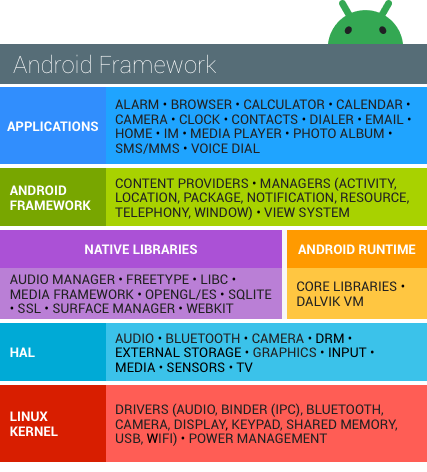
\includegraphics[scale=0.6]{inc/android-software-stack.png}
    \caption{ Программный стек Android }
    \label{fig:fig01}
\end{figure}

Таким образом, архитектура безопасности Android представляет собой целостную
систему, где каждый уровень выполняет свою роль, а шифрование служит основой
защиты пользовательских данных на всех этапах: от хранения до исполнения.

    \section{Механизмы шифрования данных в Android}

\subsection*{Полнодисковое шифрование (FDE)}

Впервые полнодисковое шифрование (full disk encryption — FDE) пытались внедрить
еще в планшетной версии Android 3.0 Honeycomb. Тогда вместе с ядром Linux
2.6.36 в ней появился модуль dm-crypt, обеспечивающий возможность шифрования на
любом блочном устройстве хранения данных (включая NAND Flash). В универсальной
четвертой версии Android шифрование также было доступно, однако для большинства
оно оставалось невостребованной опцией. Из-за отсутствия программных
оптимизаций и низкой скорости встраиваемых процессоров того времени включение
шифрования приводило к падению производительности ввода-вывода в 6–8 раз на
топовых моделях и до 20 раз на бюджетных.

Исправить ситуацию удалось только с появлением 64-битных процессоров, имеющих
отдельный набор инструкций для ускорения криптографических вычислений. Поэтому
обязательным шифрование в Android стало только с версии 5.0,
предустанавливаемой на устройства с современными однокристальными системами.

Именно в пятой версии Андроида появился флаг forceencrypt fstab, указывающий на
необходимость активации шифрования при первом включении устройства. Обрати
внимание: есть принципиальная разница между тем, было ли устройство обновлено
до Android 5.x или новее либо сразу выпускалось с такой версией. Во втором
случае шифрование данных будет выполняться всегда. В первом варианте (при
обновлении) оно останется опциональным и может быть отключено сбросом до
заводских настроек (factory reset).

В общем случае для полнодискового шифрования в Android используются три битовые
последовательности: мастер-ключ, соль и пользовательский пин-код. Мастер-ключ и
соль генерируются автоматически, а пин-код вводится владельцем устройства. Роль
пин-кода может также выполнять пароль, графический ключ или любой другой
«секрет» — для процессора это все равно битовая последовательность, причем
довольно короткая.

Пользовательские данные шифруются мастер-ключом, а соль и пин-код служат только
для того, чтобы хранить сам мастер-ключ в зашифрованном виде. Поэтому смена
пароля не приводит к перешифровке всех данных. Ключ всегда остается один и тот
же (сгенерированный изначально), а новый пароль лишь меняет его
криптографическую оболочку. Разберем эту схему подробнее.

При первом включении устройство с предустановленной ОС Android 5.0 и выше
генерирует псевдослучайный 128-разрядный ключ. Его называют мастер-ключом, или
DEK (device encryption key). Помимо DEK, также генерируется еще одно
псевдослучайное 128-битное число (соль), а пользователя просят ввести пароль.

Именно с помощью DEK в конечном счете шифруются все данные на пользовательском
разделе /data. Как именно выглядит этот ключ, владелец устройства не знает. Он
никогда не вводит его и даже не может считать штатными средствами.

В ранних версиях Android (до 5.0) мастер-ключ и настройки шифрования хранились
в отдельной незашифрованной структуре crypto footer (упрощенный аналог LUKS) в
начале зашифрованного раздела data. Сам DEX шифровался другим ключом,
вычисляемым на основе пользовательского пароля и соли.

Такой способ не обеспечивал защиту от брутфорса мастер-ключа на внешних
вычислительных системах, поэтому в Android 5.0 и выше появилось новое
требование к производителям устройств: предоставлять на аппаратном уровне
защищенное хранилище ключей. Дополнительно DEK стал подписываться с
использованием еще одного ключа (HBK — hardware-bound private key),
специфичного для данного устройства. Он захардкожен на этапе производства и не
доступен ни одному пользовательскому процессу.

Как хранение ключа, так и все ключевые криптографические процедуры в
современных версиях Android должны выполняться в изолированной среде,
недоступной пользователю и приложениям. На практике же это условие соблюдается
не всегда, поскольку Android работает на совершенно разных платформах.
Концептуально их три: ARM, Intel x86 и MIPS. В каждой из них есть свои
архитектурные ветвления, которые добавляют путаницы. Более того, на базе одних
и тех же ядер (например, ARM Cortex-A53) каждый производитель, обладающий
лицензией на архитектуру (architectural license), может сделать свою версию
однокристальной системы с любыми нестандартными свойствами.

Именно из-за такого разнообразия платформ Google до сих пор не может обеспечить
единый фундамент для шифрования, как это сделала Apple еще в 2013 году (см.
Secure Enclave). Сегодня в устройствах под управлением Android либо защищенного
хранилища ключей нет вовсе, либо оно не имеет надежной реализации.

\subsubsection*{Как работает FDE}

Поэтапно схема создания ключей для шифрования пользовательских данных в Android 5.0 и выше выглядит так:

\begin{enumerate}
    \item Гаджет при первом включении генерирует два числа длиной 128 бит. В
    дальнейшем они используются как мастер-ключ и соль.
    \item Пользователя просят задать пароль.
    \item На основе введенного пароля функция scrypt запускает формирование
    первого промежуточного ключа (IK1) длиной 256 бит.
    \item IK1 дополняется нулями так, чтобы соответствовать по длине
    аппаратному ключу HBK.
    \item Модифицированный ключ IK1 подписывается ключом HBK.
    \item Подписанный ключ IK1 используется как второй промежуточный ключ (IK2).
    \item Функция scrypt запускает формирование третьего промежуточного ключа
    (IK3), используя для его генерации IK2 и соль как входные аргументы.
    \item Первые 128 бит IK3 используются как KEK (key encryption key — ключ
    шифрования мастер-ключа).
    \item Мастер-ключ шифруется ключом KEK по алгоритму AES в режиме сцепления
    блоков шифртекста (CBC). Поскольку в данном режиме одинаковые исходные
    блоки дают одинаковый шифртекст, для затруднения атаки на основе
    подобранного шифртекста в качестве данных первого блока используется
    случайная последовательность (вектор инициализации).
    \item Зашифрованный мастер-ключ сохраняется в аппаратно изолированной области.
\end{enumerate}

Мастер-ключ используется для шифрования всего содержимого пользовательского
раздела во встроенной памяти устройства. Для каждого сектора генерируется свой
вектор инициализации с солью и указанием номера сектора (ESSIV). При вводе
пользовательского пароля мастер-ключ расшифровывается, и далее пользовательские
данные автоматически расшифровываются в фоне.

Недоступность всех ключей для прямого считывания (например, запущенным на
устройстве скриптом) обеспечивается их обработкой только внутри изолированной
доверенной среды исполнения (trusted execution environment — TEE). В
процессорах архитектуры ARM роль TEE выполняет TrustZone, которая обеспечивает
контроль целостности данных, их защищенное хранение и изолированное выполнение
кода. В ней же хранятся и промежуточные значения, вычисляемые функцией
формирования ключа.

\begin{figure}
    \centering
    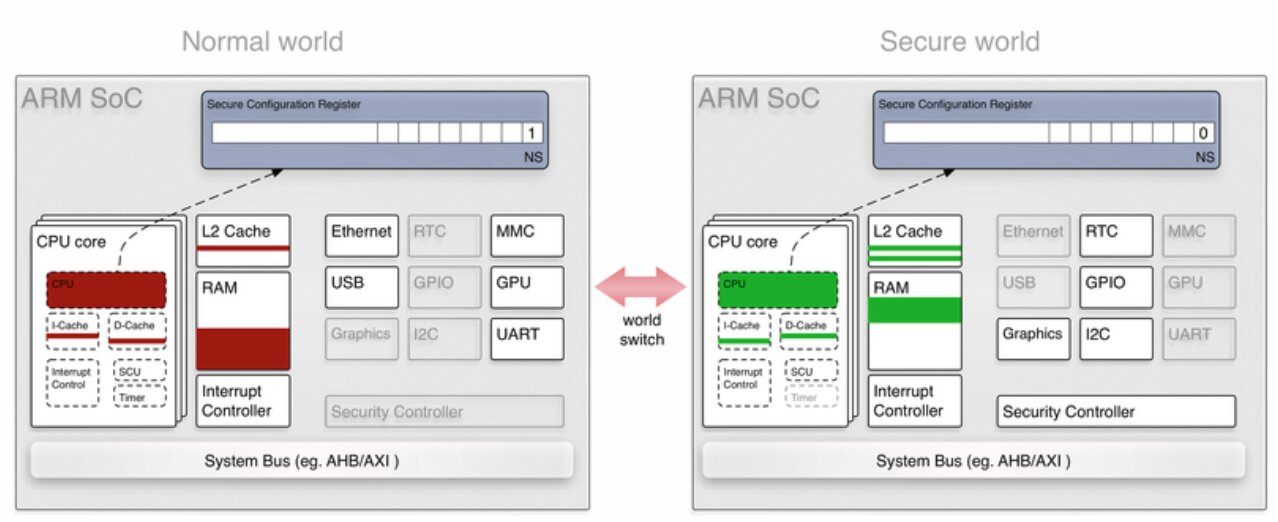
\includegraphics[scale=0.3]{inc/trustzone.jpg}
    \caption{ Схема организации доверенной среды}
    \label{fig:fig02}
\end{figure}

\subsection*{Пофайловое шифрование (FBE)}

В Android 7.0 появилась принципиально новая функция — пофайловое шифрование
(file based encryption — FBE), которое выполняется с использованием
возможностей файловой системы ext4. Новая реализация шифрования требует наличия
аппаратно изолированной среды (trusted execution environment) с поддержкой API
Keymaster 1.0 (старые версии 0.xx не годятся). Выполнение алгоритма AES
процессором должно обеспечивать расшифровку данных со скоростью не менее 50
Мбайт/с.

При использовании FBE каждый файл может быть зашифрован своим ключом и
расшифрован независимо от остальных. Эта функция работает вместе с другой
новинкой седьмого «Андроида» — прямой загрузкой (Direct Boot).

Direct Boot API обеспечивает более деликатное отделение приватных данных от
прочих файлов. Он предоставляет ту функциональность, которая была недоступна
при использовании полнодискового шифрования.

До появления Android 7.0 при активации FDE все данные хранились зашифрованными
общим паролем, поэтому смартфоном невозможно было пользоваться до ввода пароля.
Теперь же отдельные приложения (например, будильник) можно сделать доступными
прямо на экране блокировки. Они будут работать без авторизации со своими
заранее заданными ограничениями, а все пользовательские данные тем временем
останутся зашифрованными.

На устройстве с активным пофайловым шифрованием у пользователя появляется две
области хранения данных приложений: зашифрованная отдельным паролем (Credential
Encrypted — CE) и зашифрованная общим ключом устройства (Device Encrypted —
DE). При отключении FBE обе области (CE и DE) остаются открытыми для любого
приложения. При активном шифровании файлы области CE расшифровываются только
после ввода пользовательского пароля. Файлы DE могут быть расшифрованы сразу
после загрузки. Заодно раздельные пароли на каждый аккаунт позволяют создавать
на одном устройстве несколько изолированных пользовательских учеток — например,
для детей и ведущих себя подобно детям сотрудников.

Шифрование области CE происходит по алгоритму AES, но уже в другом режиме —
XTS. Он разрабатывался специально для шифрования на блочных устройствах и не
имеет типичных для режима CBC уязвимостей. В частности, XTS не позволяет
определить точку изменения данных, не подвержен утечке данных, устойчив к
атакам подмены и перемещения.

С другой стороны, FBE уязвим к side channel атакам, так как, несмотря на
шифрование файлов и их имен, он оставляет открытыми метаданные, что можно
использовать для выяснения типа хранимой информации и идентификации
пользователя устройства.

\subsection*{Android Keystore}

Одним из ключевых элементов обеспечения криптографической безопасности на
платформе Android является система \textbf{Android Keystore}. Она предназначена
для безопасного создания, хранения и использования криптографических ключей без
необходимости их извлечения в открытом виде из защищённого хранилища. Это
позволяет приложениям использовать шифрование, цифровую подпись и проверку
целостности данных без прямого доступа к самим ключам.

\subsubsection*{Назначение и архитектура}

Основная цель Android Keystore --- защитить криптографические ключи от
несанкционированного доступа и обеспечить их изоляцию от остальной части
операционной системы и приложений. Система Keystore реализована как сервис,
работающий внутри Android Framework и взаимодействующий с низкоуровневыми
компонентами устройства. На большинстве современных устройств Keystore
использует аппаратную защиту, включая:

\begin{itemize}
    \item \textbf{Trusted Execution Environment (TEE)} --- изолированная среда
    внутри процессора, в которой выполняются критические операции, включая
    криптографические.
    \item \textbf{Hardware Security Module (HSM)} --- специализированный
    аппаратный модуль для управления ключами (например, чип Titan M в
    устройствах Google Pixel).
    \item \textbf{Secure Element (SE)} --- отдельный чип, физически
    изолированный от основной системы, применяемый в некоторых устройствах для
    хранения ключей и выполнения безопасных операций.
\end{itemize}

\subsubsection*{Принцип работы}

Работа с Keystore происходит с помощью API, предоставляемого Android SDK.
Приложения могут:

\begin{itemize}
    \item Генерировать ключи асимметричного и симметричного шифрования.
    \item Выполнять операции шифрования и расшифровки данных.
    \item Подписывать и проверять цифровые подписи.
    \item Задавать условия использования ключей (например, только при разблокированном экране или только после аутентификации пользователя).
\end{itemize}

Важно, что в большинстве случаев приложение не может извлечь ключ из Keystore
--- оно может лишь передавать данные на шифрование, а сам ключ остаётся
изолированным.

\subsubsection*{Типы поддерживаемых ключей}

Android Keystore поддерживает следующие алгоритмы:

\begin{itemize}
    \item \textbf{RSA} --- асимметричное шифрование, цифровые подписи.
    \item \textbf{EC (Elliptic Curve)} --- более эффективная альтернатива RSA для цифровой подписи.
    \item \textbf{AES} --- симметричное шифрование (начиная с Android 6.0).
    \item \textbf{HMAC} --- генерация и проверка MAC-кодов.
\end{itemize}

\subsection{Условия доступа и ограничения}

Разработчики могут задать параметры для каждого ключа при его создании:

\begin{itemize}
    \item Ключ может использоваться только после прохождения биометрической или PIN-аутентификации.
    \item Ограничение по времени жизни ключа.
    \item Возможность использования только в зашифрованной области (Credential Encrypted Storage).
    \item Возможность блокировки ключа после перезагрузки устройства.
\end{itemize}

Эти условия реализуются на уровне TEE или аппаратного модуля, что делает обход этих ограничений крайне сложным даже при наличии root-доступа.

\subsubsection*{Практическое применение}

Android Keystore активно используется как в системных приложениях, так и в
стороннем программном обеспечении. Типичные сценарии использования:

\begin{itemize}
    \item Защита учётных данных (токенов, паролей) с помощью шифрования.
    \item Хранение ключей для HTTPS-соединений и VPN.
    \item Цифровая подпись и верификация целостности данных.
    \item Реализация безопасной аутентификации пользователей.
\end{itemize}

Для разработчиков Google предоставляет библиотеку
\texttt{EncryptedSharedPreferences} и \texttt{EncryptedFile}, которые
используют Keystore для защиты данных на уровне приложений.

\subsubsection*{Недостатки и ограничения}

Несмотря на высокую степень защиты, Android Keystore имеет и определённые ограничения:

\begin{itemize}
    \item Не все устройства поддерживают аппаратную реализацию Keystore; в некоторых случаях ключи хранятся в программной области.
    \item Ограниченное количество операций в секунду при аппаратной реализации.
    \item При сбросе устройства все ключи удаляются (если не использован резервный механизм).
    \item Интерфейс API может отличаться в зависимости от версии Android и производителя.
\end{itemize}

    \section{Угрозы и уязвимости}

Несмотря на многоуровневую архитектуру безопасности и активное применение
механизмов шифрования, устройства Android остаются уязвимыми перед рядом угроз.
Эти угрозы могут быть как программными, так и аппаратными, и направлены на
обход систем защиты, извлечение данных или нарушение целостности информации. В
этом разделе рассмотрим основные типы уязвимостей и приведём конкретные примеры
их эксплуатации.

\subsection{Программные угрозы}

\textbf{1. Вредоносные приложения (malware).}
Одной из самых распространённых угроз являются вредоносные приложения, которые
могут маскироваться под легитимное программное обеспечение. Они способны
похищать пользовательские данные, перехватывать нажатия клавиш, записывать
экран или аудио, а также отправлять информацию на удалённые серверы. Особенно
опасны трояны, получающие доступ к разрешениям на чтение памяти устройства.

\textit{Пример:} вирус \textbf{Joker}, обнаруженный в 2020 году, заражал
десятки приложений в Google Play и тайно подписывал пользователей на платные
услуги, похищая СМС и данные о контактах.

\textbf{2. Эскалация привилегий (Privilege escalation).}
Многие уязвимости связаны с возможностью выполнения кода с повышенными правами.
Злоумышленник может использовать эксплойты, чтобы обойти ограничения песочницы
и получить root-доступ, что даёт полный контроль над системой, включая доступ к
зашифрованным данным (при наличии ключей в оперативной памяти).

\textit{Пример:} уязвимость \textbf{Dirty COW} (CVE-2016-5195) позволяла
изменять содержимое защищённых файлов, используя гонку условий в ядре Linux.
Она применялась для получения root-доступа на Android-устройствах.

\textbf{3. Уязвимости в драйверах и прошивке.}
Драйверы оборудования и компоненты прошивки часто являются слабым звеном в
системе безопасности. Уязвимости в этих компонентах могут позволить выполнять
произвольный код до запуска системы, в обход механизмов шифрования и контроля
целостности.

\textit{Пример:} атаки на загрузчик (bootloader) позволяют заменить прошивку
или ядро, нарушив цепочку доверия Verified Boot и расшифровав пользовательские
данные.

\subsection{Аппаратные угрозы}

\textbf{1. Атаки с физическим доступом.}
Если злоумышленник получает физический доступ к устройству, он может попытаться
извлечь данные с использованием специализированного оборудования.

\textit{Пример:} \textbf{Cold Boot Attack} — техника, при которой данные из
оперативной памяти сохраняются при кратковременном отключении питания и могут
быть извлечены, включая криптографические ключи.

\textbf{2. Брутфорс PIN-кодов и паролей.}
Хотя Android ограничивает число попыток ввода пароля, при наличии аппаратных
уязвимостей можно обойти эти ограничения.

\textit{Пример:} в чипах Qualcomm Snapdragon используется собственная
реализация аппаратно изолированного окружения — QSEE (Qualcomm secure execution
environment). В нем запускаются доверенные обработчики (trustlets), включая
модуль обработки ключей (KeyMaster). Как показал этим летом Гэл Беньямини (Gal
Beniamini), в QSEE по факту нет полной аппаратной изоляции. Атакующий может
запустить свой код в пространстве QSEE. При этом он станет доверенным и
автоматически повысит привилегии, после чего сможет считать через KeyMaster как
зашифрованный мастер-ключ, так и захардкоженный ключ HBK.

Беньямини опубликовал скрипт для извлечения ключей с устройств на базе Qualcomm
Snapdragon и дальнейшие инструкции по подбору пользовательского пароля
перебором. Брутфорс не представляет сложности, так как у основной массы
пользователей короткие пароли. Поскольку атака перебором выполняется не на
смартфоне, а на любом компьютере с помощью скрипта, встроенные средства защиты
от брутфорса оказываются бессильны. При внешнем брутфорсе не возникает ни
проблем с принудительными задержками, ни риска стирания данных после N
неудачных попыток.

\textbf{3. Уязвимости в биометрических системах.}
Системы распознавания отпечатков пальцев и лица могут быть обмануты с помощью
подделок или изображений. Это особенно актуально для устройств с менее
надёжными датчиками.

\textit{Пример:} исследователи демонстрировали возможность обхода сканеров
отпечатков с помощью отпечатков, напечатанных на 3D-принтере.

\subsection{Обход шифрования}

Даже если данные физически зашифрованы, злоумышленник может попытаться получить
к ним доступ путём:

\begin{itemize}
    \item Извлечения ключей из оперативной памяти, если устройство было разблокировано.
    \item Использования уязвимостей в реализации FBE/FDE.
    \item Замены системных библиотек с целью перехвата паролей или PIN-кодов.
\end{itemize}

Кроме того, вредоносное ПО может просто получить доступ к уже расшифрованным
данным, если пользователь сам открыл устройство и дал необходимые разрешения
(например, доступ к хранилищу, камере, микрофону).

\subsection{Недостатки в реализации безопасности}

Иногда даже правильно реализованные механизмы могут страдать от ошибок
конфигурации или недостаточной строгости. Например:

\begin{itemize}
    \item Разработчики приложений могут неправильно использовать Android
        Keystore, храня ключи в открытом виде.
    \item Некоторые производители устройств отключают или модифицируют защитные
        функции (например, Verified Boot) для упрощения прошивки.
    \item Пользователи могут сами ослабить защиту, разблокировав загрузчик или
        установив root-доступ.
\end{itemize}



    \conclusion

В ходе данного исследования была подробно рассмотрена архитектура безопасности
Android и роль шифрования в защите пользовательских данных. Android как
операционная система предоставляет мощный набор механизмов для обеспечения
конфиденциальности, целостности и недоступности информации без соответствующего
доступа. Шифрование в Android является неотъемлемой частью комплексной модели
защиты, начиная с уровня ядра и заканчивая пользовательскими приложениями.

Были изучены такие ключевые технологии, как File-Based Encryption (FBE),
Android Keystore и аппаратные средства защиты (TrustZone, Secure Element, Titan
M). Особое внимание было уделено архитектуре Keystore как важнейшему компоненту
безопасного хранения ключей, и практическим последствиям разблокировки
загрузчика, что особенно актуально в контексте защиты данных при физическом
доступе к устройству.

В результате анализа угроз и уязвимостей стало очевидно, что, несмотря на
высокий уровень защиты, Android-устройства остаются подверженными рискам,
особенно при наличии root-доступа, устаревшего ПО или разблокированного
загрузчика. Практический эксперимент показал, что хотя разблокировка загрузчика
уничтожает ключи и делает невозможным восстановление ранее зашифрованных
данных, она резко снижает безопасность устройства в будущем и даёт
потенциальным злоумышленникам инструменты для модификации системы.

Таким образом, можно сделать следующие выводы:

\begin{itemize}
    \item Современные Android-механизмы шифрования являются надёжными при
        условии соблюдения стандартов безопасности.
    \item Обеспечение безопасности данных требует как технологических решений
        (шифрование, аппаратная защита), так и внимательного отношения со
        стороны пользователя (обновления, контроль разрешений, отказ от
        root-доступа).
\end{itemize}

В условиях постоянного роста цифровых угроз роль эффективного шифрования и
продуманной архитектуры безопасности будет только возрастать. Android
продолжает развиваться, внедряя всё более совершенные механизмы защиты, однако
ответственность за безопасность остаётся также и на стороне пользователя и
разработчиков приложений.

\end{document}
